\documentclass{article}
\usepackage[margin=1in]{geometry}
\usepackage{graphicx}
\usepackage{xcolor}
\usepackage{float}
\usepackage{amsmath}
\usepackage{cite}
\usepackage{hyperref}
\graphicspath{{..} {./images}}

\definecolor{navy-blue}{rgb}{0.22,0.38,0.71}

\renewcommand{\contentsname}{\vspace*{-2\baselineskip}}

\hypersetup{
	colorlinks,
	linkcolor=black,
	urlcolor=blue,
	citecolor=black
}
  		
\begin{document}
\begin{titlepage}
	\centering
	{\huge Lab 3 - Exploring the RF Spectrum}\\[0.25 in]
	
\includegraphics[width=0.6\textwidth]{ua_logo.png}\\[0.25 in]
	{\large \textbf{ECE 531 - Software Defined Radio\\[0.25 in]
	March 5, 2025\\[0.25 in]}}
	{\large Owen Sowatzke, osowatzke@arizona.edu\\[0.05 in]
	Department of Electrical \& Computer Engineering\\[0.05 in]
	University of Arizona, Tucson, AZ 85721\\[0.5 in]}
	\hypersetup{linkcolor=navy-blue}
	\noindent\hrulefill
	\tableofcontents
	\noindent\hrulefill
\end{titlepage}

\setlength{\parindent}{0pt}

\section{Introduction}
%Introduction to the laboratory experiment, including a brief description of the objectives and goals.

\section{Procedure}
% Detailed explanation of the laboratory experiment, including the design, implementation, and testing of the system.

\subsection{Identifying Signals in the RF Spectrum}

In this section, we use Fosphor to create spectrum waterfall plots of data received with the PlutoSDR. Using \url{sigidwiki.com} as a reference, we identify at least 4 different modulation techniques in received over-the-air transmissions. For each of the received signals, we describe the time and frequency characteristics that reveal the modulation technique.

\subsection{Sweeping the Spectrum: Receiving from 60 MHz to 6 GHz}

In this experiment, we perform multiple collects of the spectrum while sweeping the center frequency in steps of $F_s$. Even though our instantaneous bandwidth is limited to 56 MHz we can stitch together each of our collects to get a picture of the entire spectrum from 60 MHz to 6 GHz. This procedure is illustrated in Figure \ref{fig::sweeping_the_spectrum}. For the experiment, we specifically choose a sampling rate $F_s = 20\ \text{MHz}$. This enables us to capture the spectrum at 60 MHz even though our minimum LO frequency is 70 MHz. 

\begin{figure}[H]
	\centerline{\fbox{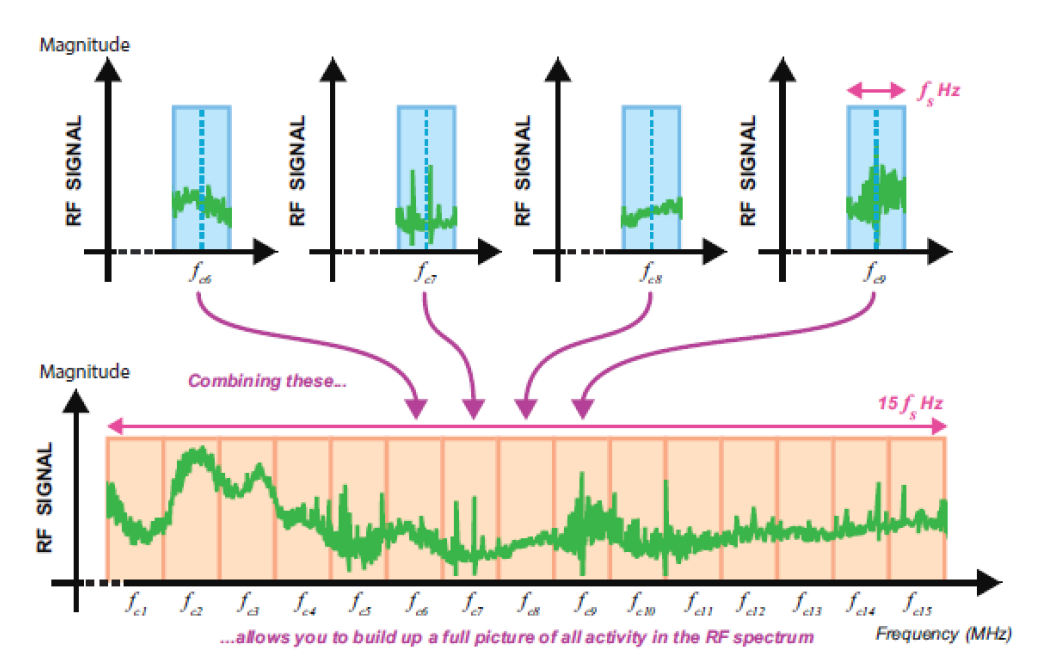
\includegraphics[width=0.7\textwidth]{sweeping_the_spectrum.png}}}
	\caption{HD Radio Spectrum}
	\label{fig::sweeping_the_spectrum}
\end{figure}

\section{Results}

% Results and discussion of the laboratory experiment, including captured outputs, observations, and responses to laboratory questions.

\subsection{Identifying Signals in the RF Spectrum}

For our first modulation technique, we looked at the FM radio band. We specifically captured data with a center frequency of 96.1 MHz and a bandwidth of 1 MHz. Our resulting collect is shown in Figure \ref{fig::hd_radio_spectrum}.

\begin{figure}[H]
	\centerline{\fbox{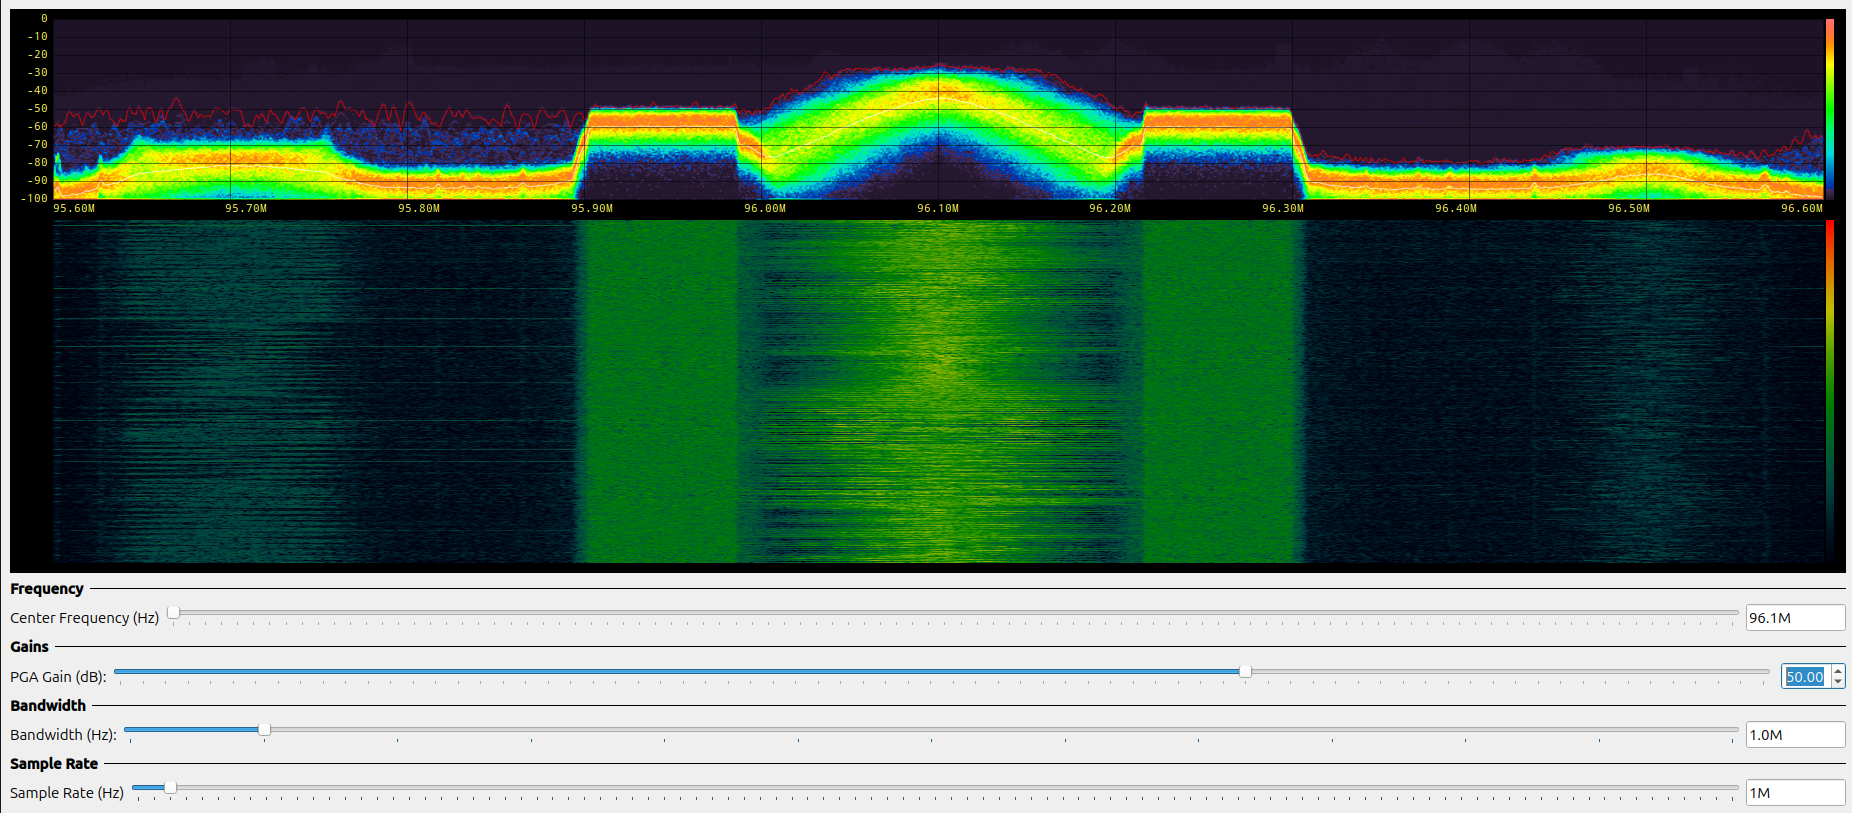
\includegraphics[width=0.7\textwidth]{hd_radio_spectrum_cropped.png}}}
	\caption{HD Radio Spectrum}
	\label{fig::hd_radio_spectrum}
\end{figure}

Note that FM radio channel we collected includes HD radio sidebands. The HD radio sidebands are digital copies of the data transmitted using OFDM modulation. The analog radio spectrum is encoded with FM modulation and rapidly oscillates in frequency with maintaining a constant amplitude. For comparison, the OFDM digital sidebands occupy fixed bandwidth and peak at approximately constant values. This is expected because OFDM encodes data into each of its subcarriers using QAM, a fixed amplitude modulation scheme. 

For our next collect, we looked at the spectrum for TV modulated with 8VSB. We specifically captured data at 485 MHz with a bandwidth of 10 MHz. Our collect is shown in Figure \ref{fig::8vsb_spectrum}.

\begin{figure}[H]
	\centerline{\fbox{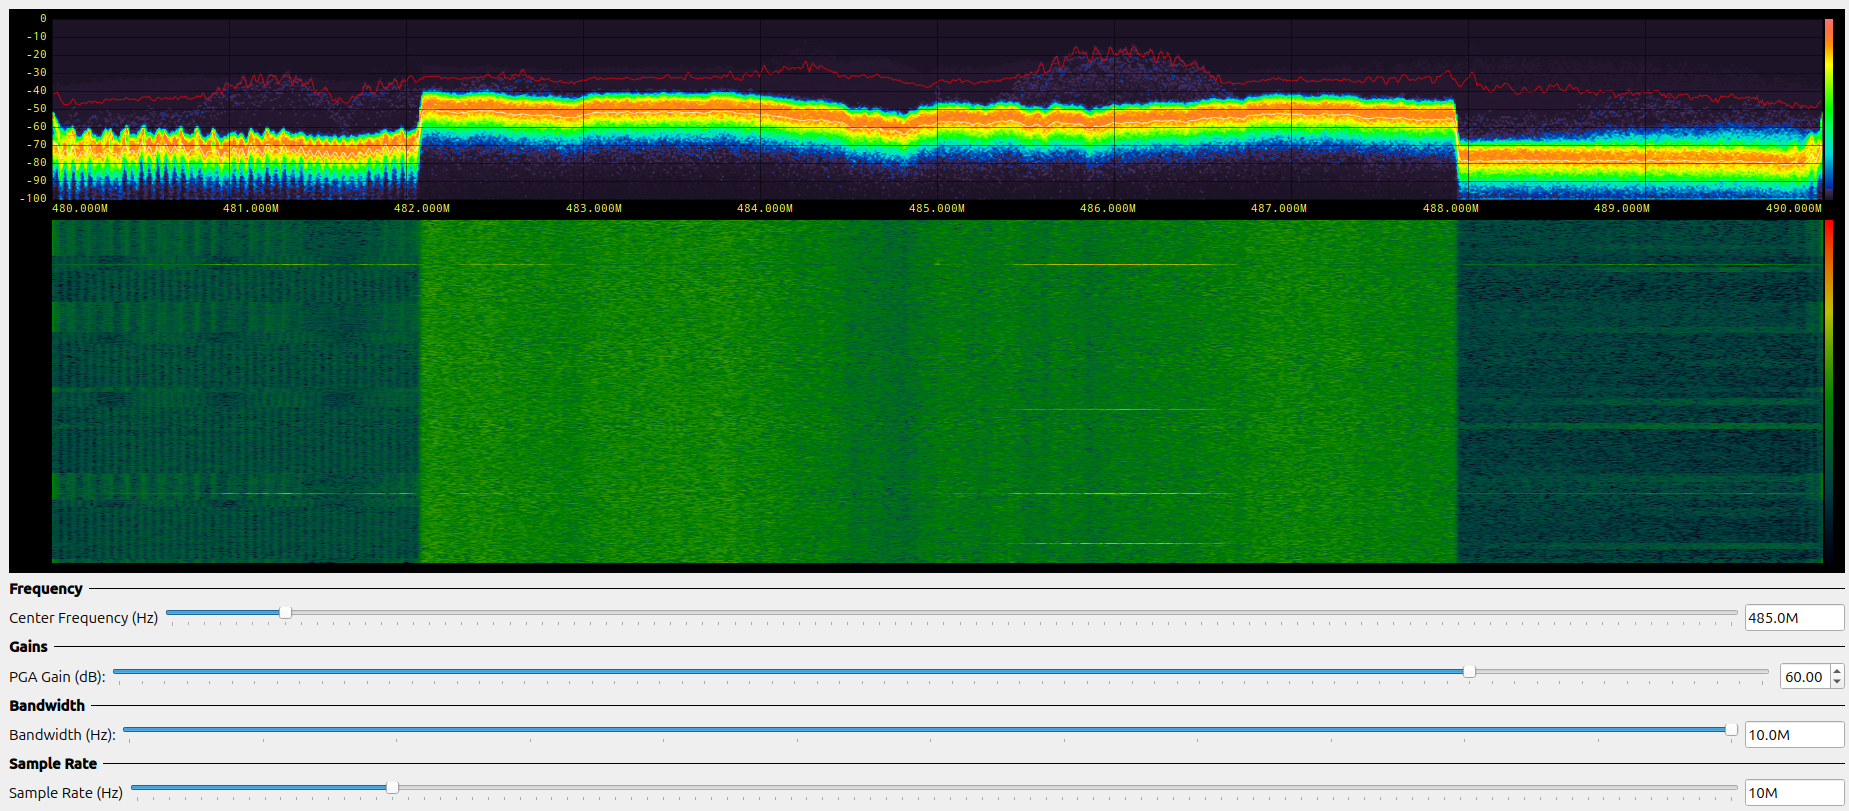
\includegraphics[width=0.7\textwidth]{8vsb_spectrum_cropped.png}}}
	\caption{Channel 16 TV Spectrum}
	\label{fig::8vsb_spectrum}
\end{figure}

8VSB uses 8 discrete levels of amplitude modulation applied digitally. It also employs a steep filter with steep cutoff to remove the sidelobes associated with the zero-order hold in the transition from discrete time to continuous time. This filter leads to a significant spectral savings.
 
Then, we looked at the LTE spectrum in the 700 MHz A spectrum. To do this, we set our center frequency to 731.5 MHz and our bandwidth to 8 MHz. The resulting spectrum is shown in Figure \ref{fig::lte_spectrum}.

\begin{figure}[H]
	\centerline{\fbox{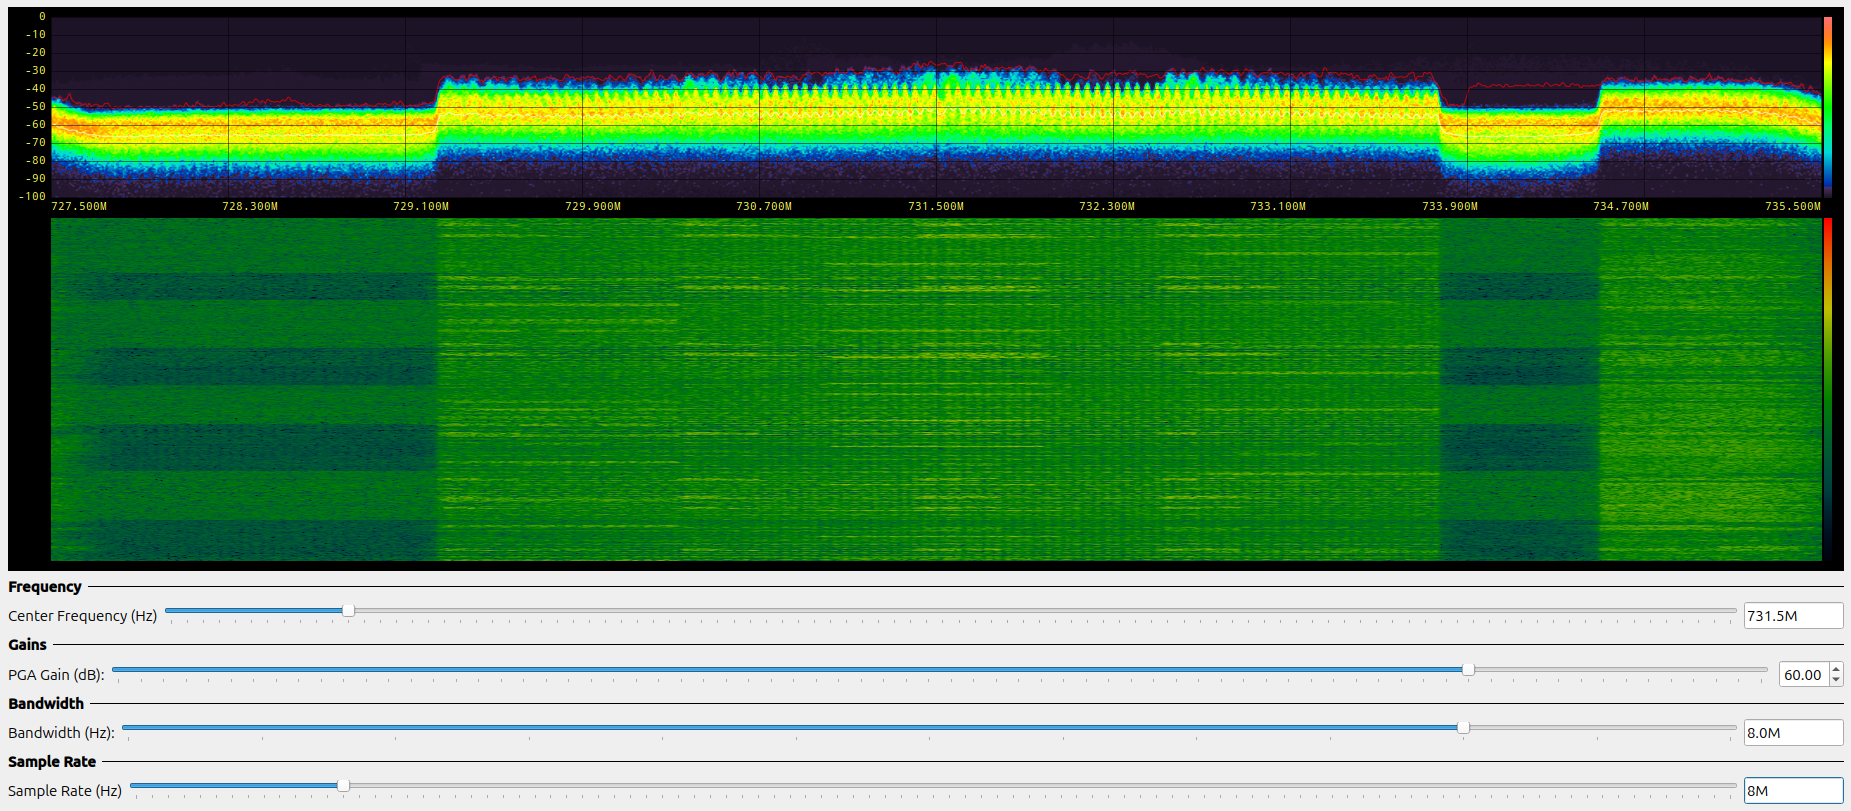
\includegraphics[width=0.7\textwidth]{lte_spectrum_cropped.png}}}
	\caption{LTE Spectrum for 700 MHz A Channel}
	\label{fig::lte_spectrum}
\end{figure}

Comparing the results to Figure \ref{fig::8vsb_spectrum}, the spectrum has much more ripple. This is expected because we are outputting tones on each of the OFDM subcarriers. Looking at time axis, we also see a lot more variation in the data due to rapidly changing symbols.

For the final modulation scheme, we looked at Motorola Type II communications in the 851 MHz - 869 MHz band, which uses FSK modulation according to \url{sigidwiki.com}. We referred to this modulation scheme instead of AM or GSM modulation because AM radio is out of band for the PlutoSDR and GSM is end of life. The resulting spectrum is shown in Figure \ref{fig::police_radio_spectrum}. It was captured with a center frequency of 851.4 MHz and a sample rate of 1 MHz.

\begin{figure}[H]
	\centerline{\fbox{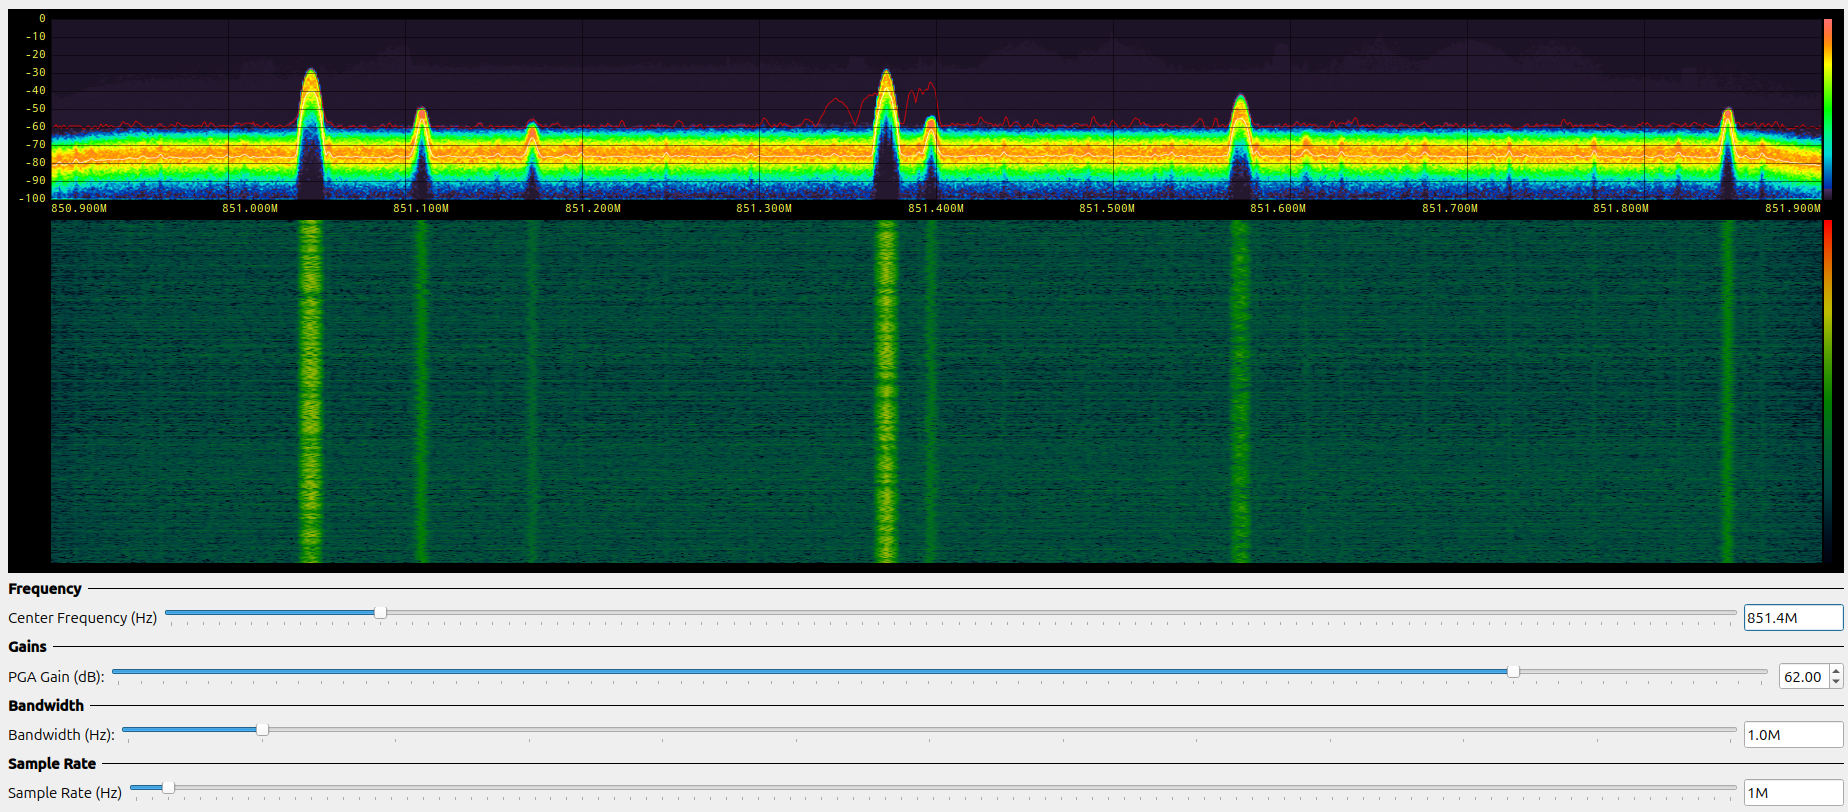
\includegraphics[width=0.7\textwidth]{police_radio_spectrum_cropped.png}}}
	\caption{Motorola Type II Spectrum}
	\label{fig::police_radio_spectrum}
\end{figure}

Motorola Type II Communications leverage multiple channels that are 12.5 kHz wide. Each of these channels use a 4 FSK modulator, which maps bits to 4 discrete frequencies. Looking at the spectrum, we see that each of these channels appear almost fixed in frequency. This is because they rapidly oscillate between each of the available frequencies.

\subsection{Sweeping the Spectrum: Receiving from 60 MHz to 6 GHz}

In this section, we stitch together multiple collects of the PlutoSDR with different center frequencies to get a picture of the frequency response from 60 MHz to 6 GHz. As previously stated, we sweep the LO frequency in 20 MHz steps. In between each collect, we call the \texttt{release} method of the \texttt{sdrrx} object. This prevents us from looking at stale data in the Pluto receive buffers. To ensure that are transmitted signal doesn't corrupt our received data, we set the LO frequency far from our collect, max-out the attenuation, and transmit zeros. After stitching together each of our collects, we get a picture of the full PlutoSDR spectrum, which we have included in Figure \ref{fig::full_spectrum_labeled}.

\begin{figure}[H]
	\centerline{\fbox{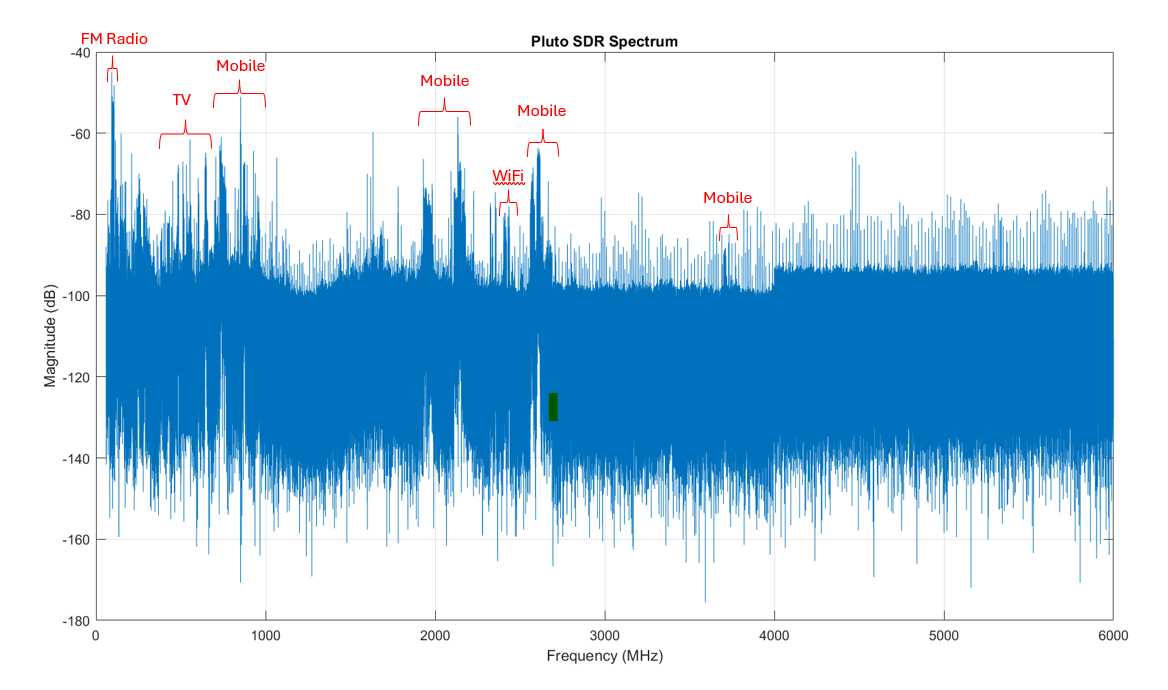
\includegraphics[width=0.7\textwidth]{full_spectrum_labeled.png}}}
	\caption{Full Pluto SDR Spectrum with Key Bands Labeled}
	\label{fig::full_spectrum_labeled}
\end{figure}

We have also labeled the key bands in the spectrum. These include FM Radio, TV, Mobile, and Wi-Fi bands. The TV bands primarily use 8VSB modulation, the Wi-Fi bands leverage OFDM in accordance with the 802.11a standard, and the mobile bands leverage mostly LTE and 5G NR.

\section{Conclusion}
% Conclusions to the overall lab that discuss meaningful lessons learned and other takeaways from the assignment. (Important)

%\nocite{analog_devices_libiio_error}
%\bibliographystyle{IEEEtran}
%\bibliography{sources}{}
%\bibliographystyle{ieeetr}
	
\end{document}